\selectlanguage{spanish}
\cover{Manual del jugador}{Imágenes al instante. Aventura con voz.}{MSX-DOS + OPL4 / v2.0}

\thispagestyle{empty}
\begin{center}\vspace*{8mm}{\fontsize{29}{33}\selectfont\bfseries\color{accent} Vuelve a la Mancha}\par\vspace{8mm}
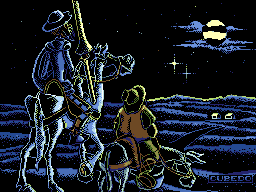
\includegraphics[width=0.85\linewidth]{assets/cover-msx2.png}
\end{center}
\textbf{Don Quijote}, publicado por Dinamic en 1987, lleva al ordenador una aventura inspirada libremente en el mundo de Cervantes. En esta aventura gráfica conversacional, Alonso Quijano persigue su ideal de caballería entre caminos, ventas y pueblos de la Mancha.

Esta edición para MSX-DOS conserva la aventura y los textos del juego existente. Puedes elegir los dibujos originales de la versión MSX1 o las ilustraciones mejoradas y la portada recoloreada de la versión MSX2. Sus novedades son la \textbf{carga rápida de las imágenes} y la \textbf{narración OPL4} de las descripciones y respuestas. Las dos partes se enlazan en una misma sesión.

Primero deberás prepararte para convertirte en caballero. Después te esperan las andanzas que te acercarán a Dulcinea. Mira a tu alrededor, lee con atención y deja que los lugares y sus habitantes te orienten.

\noteBox{Dos ediciones}{Puedes jugar en español con \cmd{QUIJOTE} o en inglés con \cmd{QUIXOTE}. Cada edición tiene sus textos, órdenes y voz en ese idioma. Los ejemplos principales de este manual corresponden a la española.}
\vfill
{\small Edición MSX-DOS + OPL4 de DiHalt Studio, 2026. Adaptación no oficial y homenaje al trabajo de sus autores originales.}
\clearpage
\tableofcontents
\vfill
\noteBox{Si ya tienes Nextor arrancado}{Copia todos los archivos de \cmd{SD/} a la carpeta del juego. Selecciona su unidad, entra en esa carpeta con \cmd{CD} y escribe \cmd{QUIJOTE}. Encontrarás el procedimiento completo en la sección de arranque en Nextor/DOS2.}

Antes de la presentación, el programa muestra la RAM compatible y la memoria de muestras OPL4 detectadas. Si los requisitos se cumplen, pulsa \key{ENTER} para continuar. Si falta memoria o no se encuentra una interfaz compatible, muestra el motivo y vuelve a DOS.

\sectionpage{Elegir español o inglés}
El idioma se elige con el archivo de arranque: \cmd{QUIJOTE.BAT} abre el menú español; \cmd{QUIXOTE.BAT}, el inglés. Después seleccionas la versión MSX1 o MSX2. Todas contienen las dos partes y funcionan en DOS1 y DOS2/Nextor.

\begin{tabularx}{\linewidth}{@{}lXX@{}}\toprule
 & Español & English\\\midrule
Carpeta de entrega & \cmd{SD/} & \cmd{SD/}\\
Orden de arranque & \cmd{QUIJOTE} & \cmd{QUIXOTE}\\
Archivos de juego & Todos; un único paquete & Todos; un único paquete\\
Narración & Español de España & Inglés británico\\\bottomrule
\end{tabularx}

Copia todos los archivos de \cmd{SD/} a una misma carpeta (a la raíz en DOS1). Contiene ambos idiomas y ambas versiones; las voces y la presentación se comparten. Escribe \cmd{QUIJOTE} o \cmd{QUIXOTE} para abrir su menú.

\begin{tabularx}{\linewidth}{@{}XX@{}}\toprule
Órdenes en español & Órdenes en inglés\\\midrule
\cmd{MIRAR}, \cmd{INVENTARIO} & \cmd{LOOK}, \cmd{INVENTORY}\\
\cmd{NORTE}, \cmd{SUR}, \cmd{ESTE}, \cmd{OESTE} & \cmd{NORTH}, \cmd{SOUTH}, \cmd{EAST}, \cmd{WEST}\\
\cmd{SUBIR}, \cmd{BAJAR} & \cmd{UP}, \cmd{DOWN}\\
\cmd{LEER LIBRO} & \cmd{READ BOOK}\\
\cmd{EXAMINAR PARED} & \cmd{EXAMINE WALL}\\
\cmd{COGER ESPADA} & \cmd{TAKE SWORD}\\
\cmd{ABRIR PUERTA} & \cmd{OPEN DOOR}\\
\cmd{ACABAR} & \cmd{QUIT}\\
\cmd{GRABAR}, \cmd{CARGAR} & \cmd{SAVE}, \cmd{LOAD}\\\bottomrule
\end{tabularx}

En inglés puedes usar \cmd{N/S/E/W/U/D}, \cmd{L} e \cmd{I}. Escribe las palabras completas de las órdenes y de los objetos, o una abreviatura admitida. Los nombres que aparecen en cada descripción te orientan.

La clave que anuncia el final de la primera parte se traduce con el juego. La pantalla inicial acepta cualquiera de las dos versiones, sin distinguir mayúsculas ni espacios. Dejarla vacía y pulsar \key{ENTER} siempre comienza la primera parte.


\sectionpage{Elegir MSX1 o MSX2}
Después de escribir \cmd{QUIJOTE} o \cmd{QUIXOTE} aparece el menú de versión. Escribe el número y pulsa \key{ENTER}.

\begin{tabularx}{\linewidth}{@{}lX@{}}\toprule
Opción & Qué ofrece\\\midrule
\cmd{1} --- MSX1 & Dibujos originales. Funciona en MSX1 o posterior.\\
\cmd{2} --- MSX2 & Ilustraciones mejoradas y portada recoloreada conservando sus formas. Requiere MSX2 o posterior.\\
\cmd{0} & Salir a DOS.\\\bottomrule
\end{tabularx}

Las dos opciones conservan la misma aventura, órdenes, voces y enlace entre las dos partes. En un MSX2 o superior puedes elegir cualquiera. En MSX1, si eliges la opción 2, el menú explica el requisito y permite elegir de nuevo.

\begin{center}
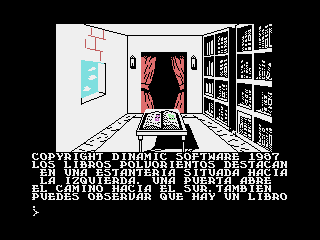
\includegraphics[width=.47\linewidth]{assets/first-room.png}\hfill
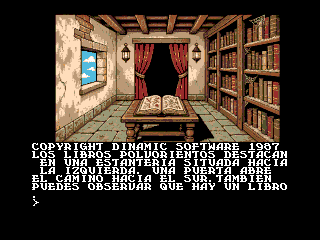
\includegraphics[width=.47\linewidth]{assets/first-room-msx2.png}\par
{\small La misma localidad en MSX1 (izquierda) y MSX2 (derecha).}
\end{center}

\noteBox{Al actualizar una instalación antigua}{Elimina los antiguos \cmd{QUIJOTE.COM} y \cmd{QUIXOTE.COM} de la carpeta antes de copiar el paquete nuevo. DOS busca los COM antes que los BAT: si quedan los antiguos, no aparecerá el menú. No borres los cuatro nuevos programas \cmd{Q1ES.COM}, \cmd{Q1EN.COM}, \cmd{Q2ES.COM} y \cmd{Q2EN.COM}.}

Si utilizas un gestor de archivos, vuelve a la consola de DOS y escribe \cmd{QUIJOTE} o \cmd{QUIXOTE}, o ejecuta expresamente el BAT de tu idioma.

\sectionpage{Lo que necesitas}
\begin{tabularx}{\linewidth}{@{}>{\bfseries}p{32mm}X@{}}\toprule
Equipo & Requisito\\\midrule
Ordenador & MSX1 o posterior para la opción 1. MSX2 o posterior para la opción 2. Teclado del MSX.\\
Almacenamiento & MegaFlashROM SCC+ SD o equivalente compatible con MSX-DOS. Se necesitan \textbf{512 KiB de RAM mapeada}.\\
Sonido & OPL4 compatible con \textbf{2 MiB de RAM para muestras}; por ejemplo, una Wozblaster con esa capacidad.\\
Sistema & MSX-DOS 1 o MSX-DOS 2 / Nextor. Los mismos menús y programas sirven en ambos.\\
Imagen & Monitor o televisor conectado a la salida habitual de vídeo del MSX.\\
Archivos & Todos los archivos de juego de \cmd{SD/}, juntos. Reserva unos \textbf{13 MiB} de espacio libre.\\
Controles & Teclado del MSX. No necesitas joystick para dar órdenes.\\\bottomrule
\end{tabularx}

La ampliación de RAM del MSX y la memoria de la OPL4 cumplen funciones distintas. \textbf{Necesitas las dos capacidades indicadas.} Comprueba la memoria instalada en tus cartuchos, no solo el nombre del modelo.

Apaga el equipo antes de conectar o retirar los cartuchos. Si utilizas más dispositivos y no quedan ranuras libres, conecta un expansor de slots adecuado para tu instalación.

\noteBox{Usa tu instalación habitual}{Arranca MSX-DOS o Nextor como haces normalmente. El juego se ejecuta desde los archivos de \cmd{SD/}; no necesitas cambiar tu sistema para seleccionar idioma o versión gráfica.}

\sectionpage{Preparar el equipo y elegir el arranque}
\begin{enumerate}
\item Con el MSX apagado, conecta la interfaz de almacenamiento y la OPL4 en ranuras disponibles.
\item Inserta la tarjeta SD que contiene los archivos del juego.
\item Conecta el monitor a la salida de vídeo habitual del MSX y prepara la salida de audio de tu equipo y de la OPL4. Empieza con un volumen moderado.
\item Enciende el monitor y el ordenador.
\item Llega al símbolo de órdenes de DOS. Si tu instalación abre un gestor de archivos, vuelve a su consola para seguir las instrucciones de arranque.
\end{enumerate}

\twochoices{archivos de juego}{Archivos en la raíz}{Archivos en una carpeta}{El mismo juego y las mismas voces}

\textbf{Nextor/DOS2} es la opción cómoda si quieres conservar el juego dentro de una carpeta. \textbf{DOS1} requiere que los archivos estén en la raíz de la partición. La letra de unidad dependerá de tu instalación: en los ejemplos usamos \cmd{B:}.

\sectionpage{Instalación y arranque en Nextor/DOS2}
Copia \textbf{todos los archivos de \cmd{SD/}} a una carpeta de tu tarjeta. Puedes llamarla \cmd{QUIJOTE} dentro de \cmd{JUEGOS}, por ejemplo.

\begin{tabularx}{\linewidth}{@{}lX@{}}\toprule
Archivo & Función para el jugador\\\midrule
\cmd{QUIJOTE.BAT}, \cmd{QUIXOTE.BAT} & Menús español e inglés.\\
\cmd{QMENU.COM} y los cuatro \cmd{Q1/Q2*.COM} & Programas de selección y juego. Copia todos.\\
\cmd{GAME.DAT}, \cmd{ENGAME.DAT}, \cmd{Q2ES.DAT}, \cmd{Q2EN.DAT} & Las dos partes en cada versión e idioma.\\
\cmd{BRAND.DAT} & Presentación de DiHalt Studio.\\
\cmd{INDEX.DAT}, \cmd{SCORES.DAT} y sus equivalentes ingleses & Recursos de la narración.\\
\cmd{VOICE0.PCM} a \cmd{VOICE5.PCM}; \cmd{ENVOX0.PCM} a \cmd{ENVOX4.PCM} & Voces de ambos idiomas, compartidas por MSX1 y MSX2.\\
\cmd{VRAM.DAT}, \cmd{VRAM.IDX}, \cmd{SC5.DAT}, \cmd{SC5.IDX} & Dibujos de las versiones MSX1 y MSX2.\\\bottomrule
\end{tabularx}

Desde la consola de Nextor/DOS2:
\begin{quote}\ttfamily
B:\\
CD \textbackslash JUEGOS\textbackslash QUIJOTE\\
QUIJOTE
\end{quote}

Ajusta \cmd{B:} y la ruta a los nombres que uses. \textbf{Debes entrar primero en la carpeta del juego}: sus datos se buscan en el directorio actual. Mantén todos los archivos juntos y con sus nombres originales.

\noteBox{Qué copiar y qué ejecutar}{Copia el contenido de \cmd{SD/}; abre \cmd{QUIJOTE.BAT} para elegir versión. Ejecuta el menú desde esa carpeta, con todos los archivos del juego juntos.}

No necesitas flashear la aventura en la MegaFlashROM. Se ejecuta desde los archivos de la SD.

\sectionpage{Instalación y arranque en DOS1}
\textbf{DOS1 no admite subdirectorios.} Copia todos los archivos de \cmd{SD/} a la \textbf{raíz} de la unidad desde la que vas a jugar. Conserva sus nombres y mantén juntos los programas, las imágenes y las voces de ambos idiomas.

Arranca tu instalación habitual de DOS1. Selecciona la unidad que contiene el juego y escribe el menú de tu idioma:
\begin{quote}\ttfamily
B:\\
QUIJOTE
\end{quote}
Para inglés, escribe \cmd{QUIXOTE}. La letra \cmd{B:} es un ejemplo; utiliza la que corresponda a tu disco o tarjeta.

\begin{tabularx}{\linewidth}{@{}lX@{}}\toprule
En DOS1 & Qué debes hacer\\\midrule
Ubicación & Todos los archivos directamente en la raíz de la unidad.\\
Idioma & \cmd{QUIJOTE.BAT} para español o \cmd{QUIXOTE.BAT} para inglés.\\
Versión gráfica & Opción \cmd{1} para MSX1 o \cmd{2} para MSX2, seguida de \key{ENTER}.\\
Datos & Copia todos los archivos de \cmd{SD/}; no mezcles archivos de distintas ediciones.\\\bottomrule
\end{tabularx}

\noteBox{El mismo paquete para ambos DOS}{DOS1 y Nextor/DOS2 utilizan los mismos archivos del juego. Cambia su ubicación: raíz para DOS1, raíz o carpeta para Nextor/DOS2. La selección de idioma y versión funciona igual.}

Una vez elegido el programa, confirma el informe de memoria con \key{ENTER}. Si falta un requisito, lee el mensaje y vuelve a DOS para revisar tu configuración antes de iniciar otra vez el juego.

\sectionpage{Del arranque a tu primera orden}
Tras elegir versión y confirmar con \key{ENTER} el informe de memoria, verás la presentación de DiHalt Studio acompañada por una fanfarria OPL4 de unos diez segundos. Al terminar, pulsa \key{ENTER} con la entrada vacía para empezar la primera parte, o escribe la clave obtenida al completarla para empezar la segunda. Puedes corregirla con \key{BS}; si no es válida, vuelve a intentarlo. Después aparece la portada. Se mantiene en pantalla hasta que pulses una tecla para comenzar la parte elegida.

Cuando entres en una localidad con dibujo, \textbf{la imagen se muestra primero}; a continuación aparecen la descripción y su narración. Espera a que termine la frase, o pulsa \key{ESC} para cancelarla, antes de escribir tu orden.

\screenfigure{La primera localidad: el dibujo, la descripción y el indicador de entrada del juego original.}

\begin{enumerate}
\item \textbf{Dibujo}: muestra el lugar cuando existe una ilustración para esa localidad.
\item \textbf{Texto}: describe las salidas, los objetos y las consecuencias de tus acciones.
\item \textbf{Entrada}: el símbolo \cmd{>} indica dónde puedes escribir tu siguiente orden.
\end{enumerate}

Cuando completes la primera parte, atiende al aviso y pulsa una tecla cuando se te pida. La segunda parte se carga en la misma sesión, \textbf{sin volver a escribir la clave}. Su portada también espera una tecla antes de continuar. Anótala para comenzar directamente en la segunda parte en otra sesión; no recupera una partida intermedia.

\sectionpage{Controles y órdenes}
\begin{tabularx}{\linewidth}{@{}p{43mm}X@{}}\toprule
Acción & Tecla u orden\\\midrule
Escribir una orden & Letras, espacios y nombres de objetos. Se admiten minúsculas.\\
Enviar la orden & \key{RETURN / ENTER}\\
Corregir al escribir & \key{BS / Retroceso}\\
Cancelar la frase hablada & \key{ESC}; suelta la tecla antes de cancelar otra frase.\\
Volver a describir el lugar & \cmd{MIRAR} (también \cmd{M}).\\
Consultar lo que llevas & \cmd{INVENTARIO} (también \cmd{I}).\\
Moverte & \cmd{NORTE}, \cmd{SUR}, \cmd{ESTE}, \cmd{OESTE}, \cmd{SUBIR}, \cmd{BAJAR}, cuando exista ese paso.\\
Reiniciar la aventura & \cmd{ACABAR}. Úsalo si quieres volver a empezar.\\\bottomrule
\end{tabularx}

Cada orden admite \textbf{31 caracteres, incluidos los espacios}: una sola línea. Al llenarla, no se añaden más caracteres. Puedes usar \key{BS / Retroceso} para corregir o \key{RETURN / ENTER} para enviarla.

La forma más sencilla de dar una instrucción es \textbf{verbo + nombre}:
\begin{quote}
\cmd{LEER LIBRO}\par
\cmd{EXAMINAR PARED}\par
\cmd{COGER ESPADA}\par
\cmd{ABRIR PUERTA}
\end{quote}
Escribe las órdenes sin tildes, como en estos ejemplos. Son muestras de vocabulario del juego, no una secuencia que debas seguir. El lugar, los objetos que llevas y lo ocurrido anteriormente determinan si una acción tiene sentido.

\noteBox{Si escribes mientras habla}{La escritura normal se atiende después de la narración. Espera o cancela la frase con \key{ESC}; luego escribe y pulsa \key{RETURN / ENTER}.}


\sectionpage{Cómo avanzar sin perderte}
Lee la descripción completa antes de actuar. A menudo contiene la salida que buscas o una pista sobre algo que merece examinarse. Si quieres escuchar o leer de nuevo el lugar, utiliza \cmd{MIRAR}.

\begin{itemize}
\item \textbf{Explora con método.} Anota las direcciones y dibuja un pequeño mapa de las localidades que ya conoces.
\item \textbf{Observa y lee.} Un objeto puede tener información útil aunque todavía no puedas llevártelo.
\item \textbf{Revisa el inventario.} El espacio y los objetos que conservas importan; el juego te avisará si llevas demasiadas cosas.
\item \textbf{Prueba acciones concretas.} Si la respuesta no es la que esperabas, revisa el verbo, el objeto y el lugar en que te encuentras.
\item \textbf{Cuida al hidalgo.} Comer y descansar forman parte de la aventura. Atiende a los avisos del juego.
\item \textbf{No todo se ve de inmediato.} La oscuridad y las circunstancias de una escena pueden limitar lo que puedes observar.
\end{itemize}

\begin{center}\begin{tikzpicture}[font=\small,n/.style={draw=accent,fill=paper,rounded corners,text width=26mm,align=center,minimum height=12mm},a/.style={-Latex,thick,draw=teal}]
\node[n] (m) {Mirar};\node[n,right=6mm of m] (e) {Examinar};\node[n,right=6mm of e] (p) {Pensar};\node[n,right=6mm of p] (a) {Actuar};
\draw[a](m)--(e);\draw[a](e)--(p);\draw[a](p)--(a);
\end{tikzpicture}\end{center}

\noteBox{Sobre guardar y cargar}{Esta edición no incorpora partidas guardadas en la SD. Las órdenes originales \cmd{GRABAR} y \cmd{CARGAR} conservan el funcionamiento de cinta de la versión MSX. No las utilices esperando crear o abrir un archivo de partida en la carpeta del juego.}

La ilustración no sustituye al texto. Algunas localidades pueden carecer de dibujo; sigue leyendo las descripciones y las respuestas para decidir qué hacer.

\sectionpage{Si algo no funciona}
\begin{tabularx}{\linewidth}{@{}p{47mm}X@{}}\toprule
Lo que ocurre & Qué comprobar\\\midrule
DOS no encuentra \cmd{QUIJOTE} & Selecciona la unidad correcta. En DOS2/Nextor, entra con \cmd{CD} en la carpeta que contiene \cmd{QUIJOTE.BAT}.\\
Error al cargar recursos & Comprueba todos los archivos y sus nombres. En DOS1 deben estar en la raíz; en DOS2, todos en el directorio actual.\\
No aparece el menú al actualizar & Borra los antiguos \cmd{QUIJOTE.COM} y \cmd{QUIXOTE.COM}; conserva los nuevos BAT y todos los archivos del paquete.\\
El programa se ve, pero no se oye & Comprueba la conexión y el volumen de la OPL4, su salida de audio y que dispone de 2 MiB de RAM para muestras.\\
Las letras no aparecen mientras habla & Espera a que termine la frase o pulsa \key{ESC}. Después escribe la orden.\\
La orden no se entiende & Usa vocabulario español y frases sencillas. Comprueba el nombre del objeto y vuelve a examinar el lugar.\\
La partida vuelve a empezar & Lee el último aviso. Algunas acciones o situaciones ponen fin al intento.\\\bottomrule
\end{tabularx}





\sectionpage{Créditos y derechos}
\textbf{Juego original}\par
Don Quijote, Dinamic Software, 1987.\par
Programa: \textbf{Jorge Blecua (Egroj)}.\par
Versión MSX: \textbf{Marcos Jourón Berzosa}.\par
Gráficos: \textbf{Pablo y Egroj}.\par
Pantalla de carga: \textbf{Javier Cubedo}.\par
Diseño artístico: \textbf{Ángel Luis González}.

\textbf{Edición MSX-DOS + OPL4}\par
\textbf{DiHalt Studio, 2026}: adaptación de carga desde SD, enlace de las dos partes, carga rápida de imágenes, versión gráfica MSX2, narración OPL4 y este manual. Conserva los textos y la aventura de los autores originales.

Este proyecto es una adaptación no oficial y un homenaje. Don Quijote, sus gráficos, textos y demás elementos originales pertenecen a sus respectivos titulares. No se declara afiliación con Dinamic ni con los autores originales. La presente edición no otorga derechos sobre las obras originales.

Las imágenes de este manual proceden del propio juego: portada firmada por Cubedo y captura de la primera localidad. El logotipo MSX es una marca de sus titulares; la imagen procede del logotipo de formas simples publicado en Wikimedia Commons. El logotipo DiHalt Studio pertenece al proyecto.

\textbf{Lecturas y procedencia}\par
La ficha, los créditos y la reproducción del manual original conservados por Computer Emuzone se utilizaron para contrastar la historia y los nombres:\par
\href{https://computeremuzone.com/ficha/151/don-quijote}{computeremuzone.com/ficha/151/don-quijote}.\par
El archivo \cmd{SOURCES.md}, junto a las fuentes de este manual, detalla la procedencia de cada ilustración y de la información consultada.

\vfill
\textcolor{accent}{\textbf{Conserva la aventura. Comparte tus observaciones.}}\par
Código fuente y documentación disponibles en el \href{https://github.com/DiHaltStudio/donquijote-msx1-opl4-en-es}{repositorio de GitHub de DiHalt Studio}. ¡Mejora el juego si te apetece!
